% !TEX root = ../main.tex
%

\section{Results}
\label{sec:results}

\subsection{Main findings}

\begin{enumerate}[nosep, noitemsep]
    \item Unmoderated discussions exhibit significantly higher toxicity and lower \ac{AQ} (Figure \ref{fig::toxicity_aq_stats}) (ANOVA $p<.000$).

    \item  While the Moderation and Facilitation Guidelines slightly improve \ac{AQ} relative to baselines, their impact is marginal (Figure \ref{fig::toxicity_aq_stats}). Notably, these strategies do not reduce toxicity more effectively than the “No Instructions” baseline and perform worse than the “Rules Only” strategy.

    \item Toxicity and \ac{AQ} generally improve over time under all strategies when compared to unmoderated discussions, indicating a limited but consistent restraining effect over time (Table \ref{tab:timeseries}).

    \item \ac{LLM} moderators intervene frequently throughout discussions (Figure \ref{fig::intervention_count}). \ac{LLM} user-agents exhibit an atypical tolerance for excessive moderator interventions, whereas with human participants such repeated interventions often provoke irritation and increased toxicity \cite{schaffner_community_guidelines, make_reddit_great, proactive_moderation, cresci_pesonalized_interventions}.
\end{enumerate}


\begin{figure*}[t]
    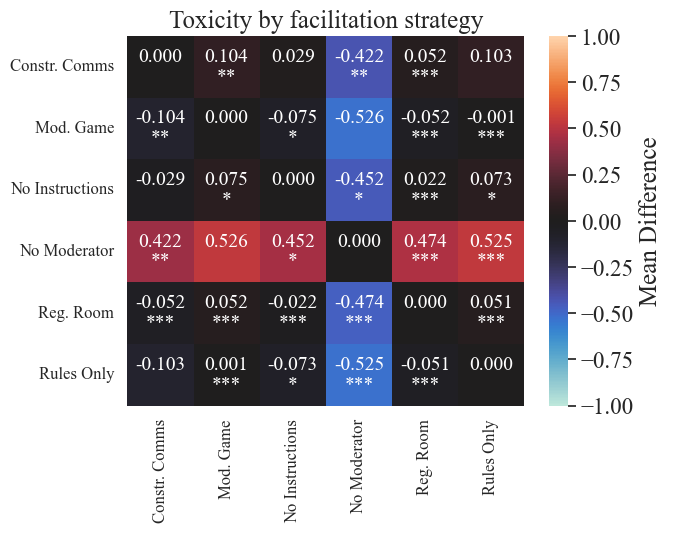
\includegraphics[width=0.48\linewidth]{toxicity_stats.png} \hfill
    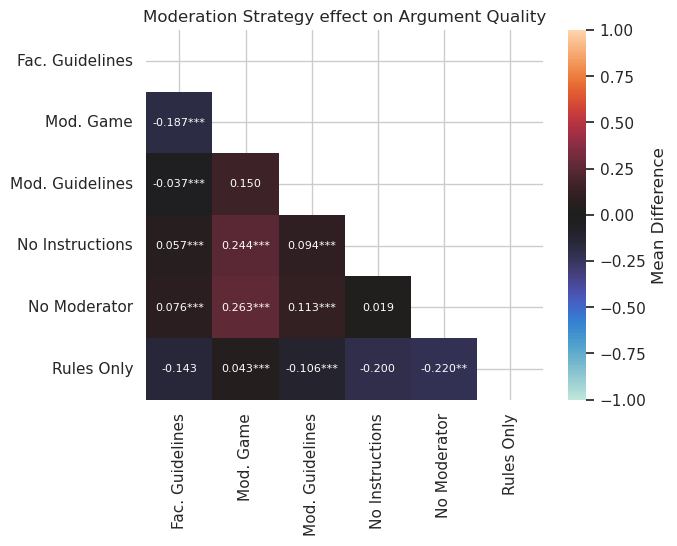
\includegraphics[width=0.48\linewidth]{argumentq_stats.png}
	\centering
	\caption{Mean difference of Toxicity (left) and \ac{AQ} (right) between each moderation strategy. $A[i, j] = 0.3^{***}$ indicates that the strategy $i$ leads to overall worse discussions (more toxicity/worse arguments) compared to $j$ for an average of $0.3$ points with $p<0.001$. Each comparison is accompanied by pairwise student-t tests, in the form of significance asterisks.}
	\label{fig::toxicity_aq_stats}
\end{figure*}

\begin{figure}
	\centering
	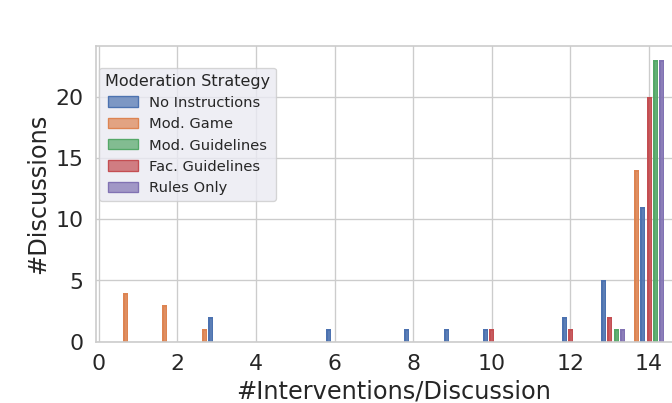
\includegraphics[width=\columnwidth]{intervention_count.png}
	\caption{Histogram of interventions by \ac{LLM} moderators. The maximum number of interventions is $14$.}
	\label{fig::intervention_count}
\end{figure}

\begin{table}[htbp]
    \centering
    \begin{tabular}{lll}
        \toprule
        \textbf{Variable} & \textbf{Toxicity} & \textbf{Arg.Q.} \\
        \midrule
        Intercept & 2.164\textsuperscript{***} & 2.113\textsuperscript{***} \\
        Fac. Guid. & -0.230\textsuperscript{***} & -0.007 \\
        Mod. Guid. & -0.277\textsuperscript{***} & -0.107\textsuperscript{*} \\
        \ac{RL} Game & -0.435\textsuperscript{***} & -0.282\textsuperscript{***} \\
        No Instructions & -0.426\textsuperscript{***} & -0.213\textsuperscript{***} \\
        Rules Only & -0.461\textsuperscript{***} & -0.305\textsuperscript{***} \\
        time & -0.012\textsuperscript{**} & -0.012\textsuperscript{**} \\
        Fac. Guid:time & -0.023\textsuperscript{***} & -0.024\textsuperscript{***} \\
        Mod. Guid:time & -0.023\textsuperscript{***} & -0.011\textsuperscript{*} \\
        \ac{RL} Game:time & -0.011\textsuperscript{*} & 0.003 \\
        No Instructions:time & -0.003 & 0.003 \\
        Rules Only:time & -0.008 & -0.002 \\
        \bottomrule
    \end{tabular}
    \small
    $\cdot p<0.1$, \textsuperscript{*} $p<0.05$, \textsuperscript{**} $p<0.01$, \textsuperscript{***} $p<0.001$
    \normalsize
    \caption{OLS Regression Coefficients for Toxicity ($Adj. R^2=0.054$) and \ac{AQ} ($Adj. R^2=0.016$). \textit{“Time”} denotes dialogue turn, reference factor is \textit{“No moderator”}.}
    \label{tab:timeseries}
\end{table}



\subsection{Ablation study}
\label{ssec:results:ablation}

We test the effects of our proposed methodology by running $8$ synthetic discussions using the Qwen 2.5 model, and comparing their \textit{diversity} scores (Section \ref{ssec:methodology:diversity}) with our original dataset, as well as with human discussions. We use the Cornell eRulemaking “Regulation Room” dataset \footnote{\url{http://archive.regulationroom.org}}, from which we extract all comments from all initiatives. We assert that diversity distributions closer to the ones observed in the human discussions indicate they are realistic.

% Any opinions, findings, and conclusions or recommendations expressed in this material are those of the author(s) and do not necessarily reflect the views of the CeRI (Cornell e-Rulemaking Initiative)


\subsubsection{Models}

The Qwen 2.5 model is the model with the most observed \textit{diversity} (see Section \ref{ssec:methodology:diversity}), followed by the Mistral Nemo and the LLaMa 3.1 model (Figure \ref{fig::diversity}). However, maximizing diversity should not be our goal, since a theoretical discussion where participants ignore each other and talk about unrelated subjects would have very high diversity scores. Both the Mistral and Qwen models somewhat approximate the observed diversity of human discussions, which may indicate that large models subjected to intense alignment procedures may not be able to replicate human behavior as authentically as other models (as reported in \citet{Park2023GenerativeAI}). 

Alternatively, LLaMa's longer comments (Figure \ref{fig::comment_length}) may have caused the higher diversity scores. We find a qualitatively significant  ($Adj. R^2=0.202$), positive correlation ($\textit{diversity} = 2.38\mathrm{e}{-05} \times \textit{\#words} \times \textit{is\_synthetic} + 0.9030$) between the length of \textit{synthetic} discussions and their diversity score.


\subsubsection{Turn taking}

We investigate three turn taking functions: The Round Robin algorithm, which gets each user to talk in a predetermined, unchanging order, random selection, and our proposed turn taking algorithm (Section \ref{ssec:experimental:turn}).

While the turn taking function by itself is not enough to approximate the human discussions (Figure \ref{fig::diversity} — since all the distributions diverge from the human distribution), it still seems to improve synthetic discussions. Discussions where the turn to speak was given either by chance or rotation, demonstrate extremely high diversity scores, diverging significantly from the human diversity distribution. This can not be explained by comment length (Figure \ref{fig::comment_length}). Thus, our proposed turn taking algorithm meaningfully positively impacts the quality of the generated data.


\subsubsection{Prompting}

We run discussions where user-agents (1) are not assigned \acp{SDB}, (2) are not assigned roles, and (3) are given a baseline prompt (see Appendix \ref{sssec:appendix:actors}). Figure \ref{fig::diversity} demonstrates that, while our approach (using roles, \acp{SDB} and the improved instruction prompt) is not enough to create discussions with similar diversity as human ones, removing any of its aspects leads to a significant divergence. This divergence is similar to the one observed when changing the turn taking function, and can similarly not be attributed to differences in comment length (Figure \ref{fig::comment_length}).

Finally, we test whether user-agents assigned with the “Troll” role lead other user-agents into displaying toxic behavior. We find that discussions which involved trolls cause a statistically and qualitatively significant rise in toxicity in the comments of the rest of the user-agents (Student-t test $p<.000$, see Figure \ref{fig::goad}). This was to be expected, since we explicitly set this behavior in our instruction prompt.

\begin{figure}
    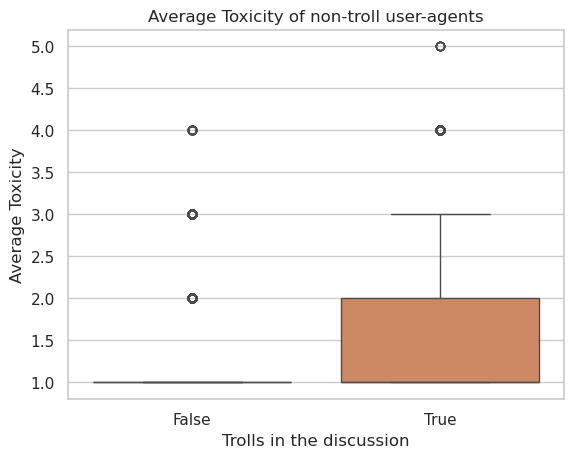
\includegraphics[width=\columnwidth]{toxicity_troll_comparison.png} 
	\caption{Trolls cause other participants to display toxic behavior.}
	\label{fig::goad}
\end{figure}

\begin{figure*}[t]
    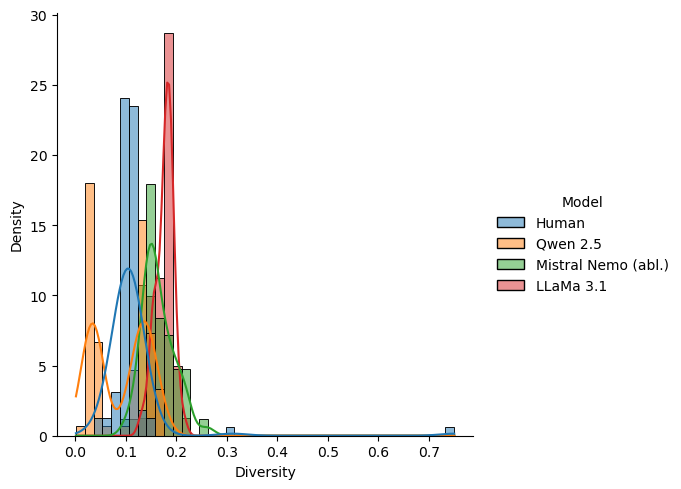
\includegraphics[width=0.30\linewidth]{rougel_model.png} \hfill
    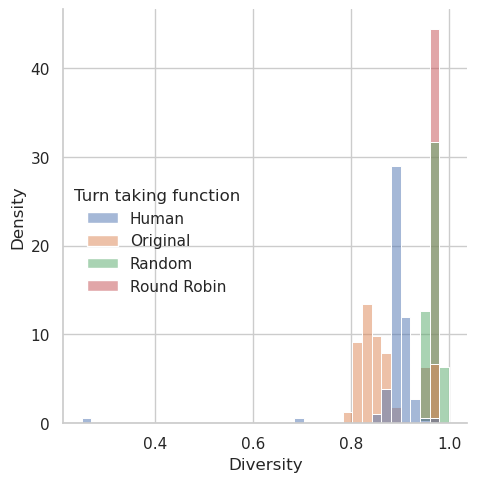
\includegraphics[width=0.30\linewidth]{rougel_turns.png}
    \hfill
    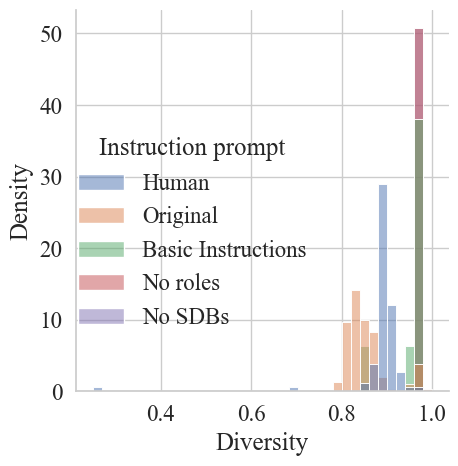
\includegraphics[width=0.30\linewidth]{rougel_prompts.png}
	\centering
	\caption{Diversity (Section \ref{ssec:methodology:diversity}) distribution for each discussion by model (Section \ref{ssec:experimental:model}), turn-taking function $u$ (Section \ref{ssec:experimental:turn}), and prompting function $\phi$ used (Section \ref{ssec:experimental:prompts}).}
	\label{fig::diversity}
\end{figure*}

\begin{figure*}[t]
    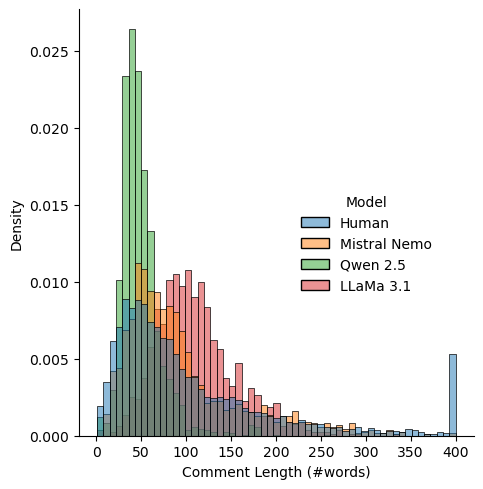
\includegraphics[width=0.30\linewidth]{comment_len_model.png} \hfill
    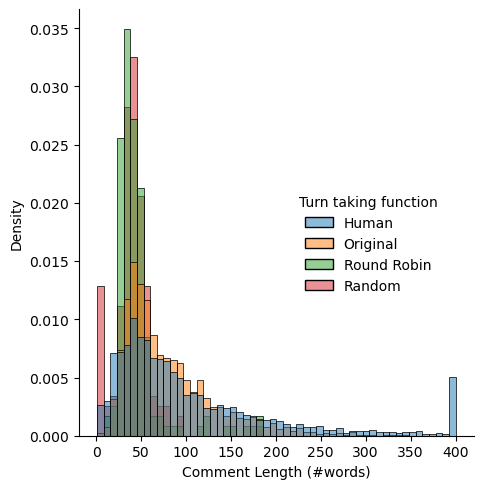
\includegraphics[width=0.30\linewidth]{comment_len_turns.png}
    \hfill
    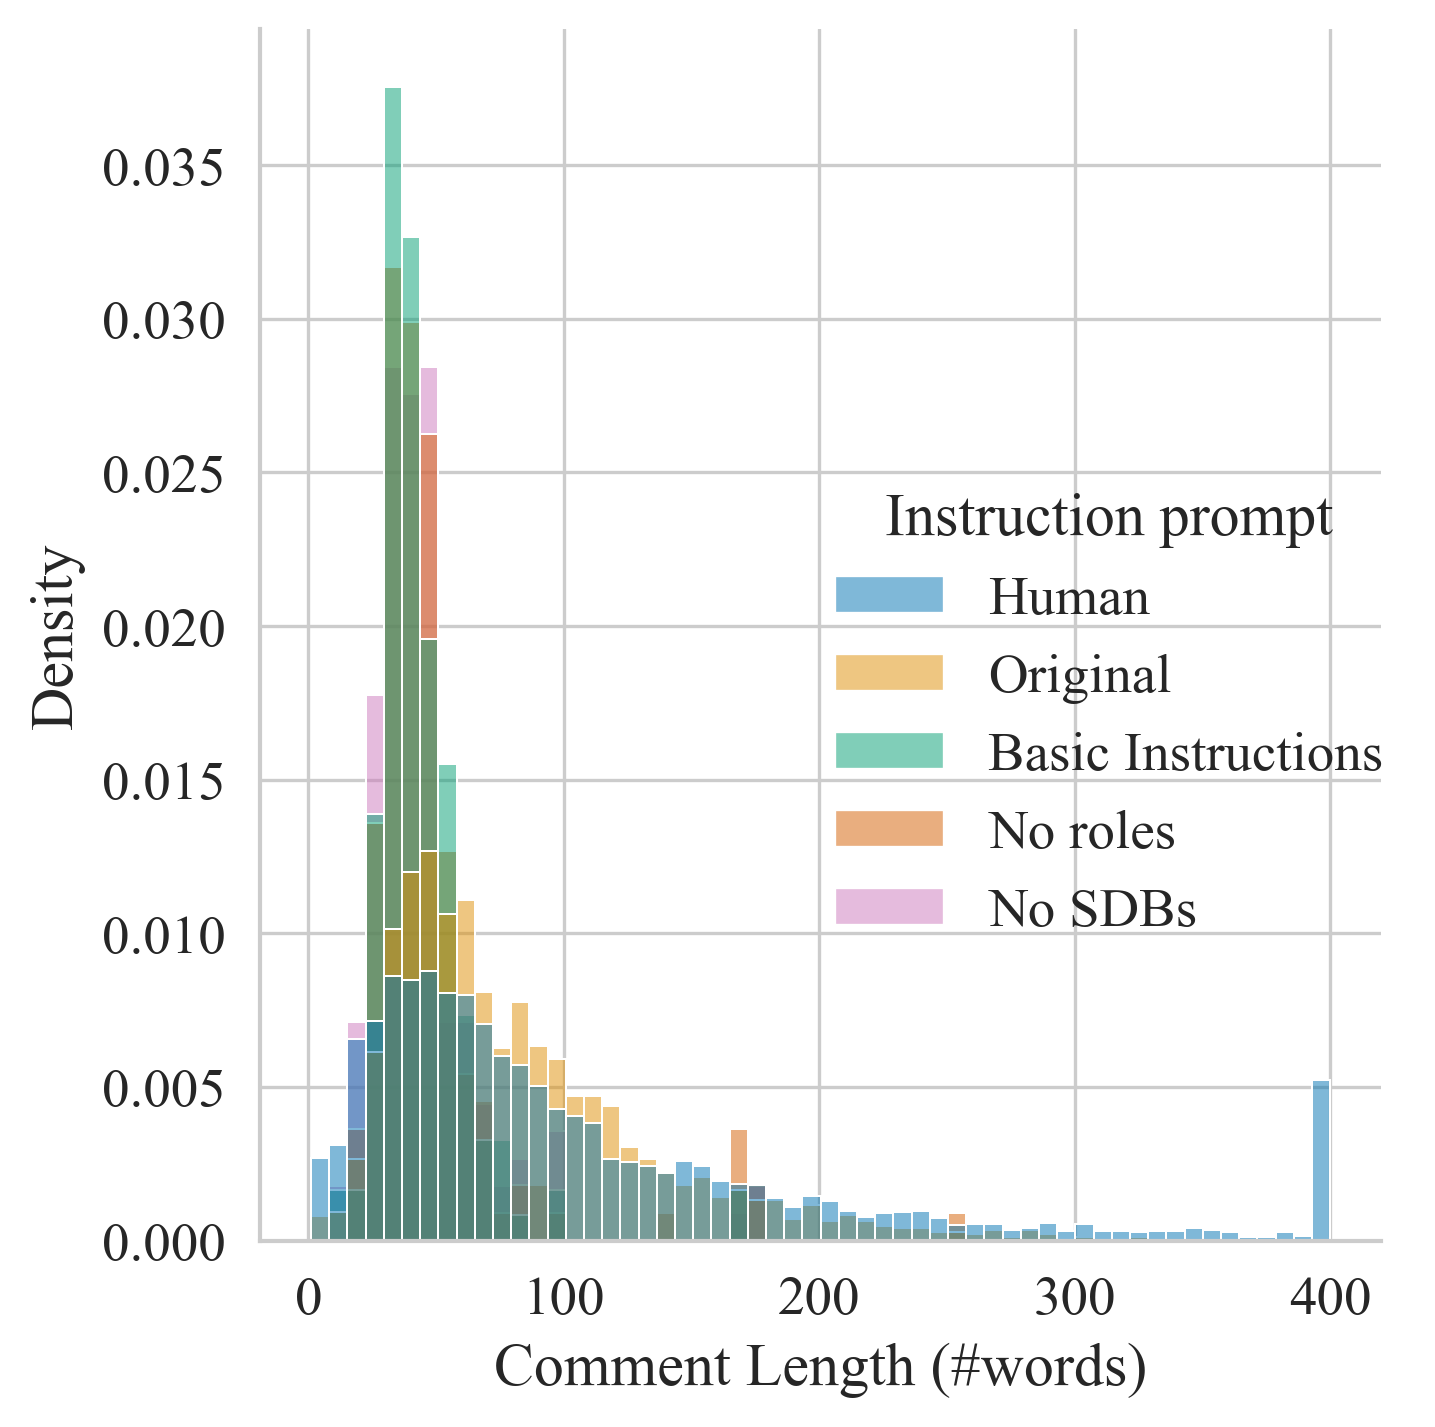
\includegraphics[width=0.30\linewidth]{comment_len_prompts.png}
	\centering
	\caption{Comment length for each discussion by model (Section \ref{ssec:experimental:model}), turn-taking function $u$ (Section \ref{ssec:experimental:turn}), and prompting function $\phi$ used (Section \ref{ssec:experimental:prompts}). For ease of comparison, comments above $400$ words are marked at the end of the x-axis.}
	\label{fig::comment_length}
\end{figure*}



